%----------------------------------------------------------------------
\chapter[A brief introduction to astrodynamics]{A brief introduction to astrodynamics}
%----------------------------------------------------------------------
 
We usually refer to celestial mechanics, astrodynamics, orbital dynamics, attitude dynamics or astronomy as the same thing. However it is important to make clear that these concepts differ from each other and we should properly understand what we refer to when talking about each one. Let us start this chapter by defining them in detail:

\vspace{0.25cm}
\begin{Definition*}{}
	\textbf{Celestial mechanics} is the scientific study of celestial body dynamics.
\end{Definition*}
\vspace{0.25cm}

\vspace{0.25cm}
\begin{Definition*}{}
	\textbf{Orbital dynamics} is the scientific study of the motion of small orbiting bodies.
\end{Definition*}
\vspace{0.25cm}

\vspace{0.25cm}
\begin{Definition*}{}
	\textbf{Attitude dynamics} is the scientific study of the relative position and orientation of bodies in space.
\end{Definition*}
\vspace{0.25cm}

\vspace{0.25cm}
\begin{Definition*}{}
	\textbf{Astronomy} is  the scientific study of matter and phenomena in the universe, especially in outer space, including the positions, dimensions, distribution, motion, composition, energy, and evolution of celestial objects.
\end{Definition*}
\vspace{0.25cm}

\begin{Definition*}{}
	\textbf{Astrodynamics} is the branch of astronomy that studies the motion of celestial and man-made bodies in space subjected to both natural and artificial perturbations.
\end{Definition*}
\vspace{0.25cm}

\section{The Solar System models}

When first human beings started to look at the stars, they tried to explain 

\begin{figure}[h]
	\centering
	\includegraphics[scale=0.75]{figs/sky_path.png}
	\caption{Apparent path of a celestial body}
\end{figure}


\newpage
\section{Solar System bodies}

\begin{figure}[h]
	\centering
	\includegraphics[scale=0.85]{figs/bodies/mercury.png}
	\caption{Mercury data}
\end{figure}